%%% Removed from symbolic_dynamics.tex
%\documentclass[12pt,twoside]{book}
%\usepackage{../../thesis}
%\graphicspath{ {../../images/} }
%
%\makeindex
%\begin{document}
\chapter{Symbolic Dynamics}
\section{Invariant Set of The Horseshoe Map}
The treatments of the horseshoe map and symbolic dynamics follows \citet{wiggins}.
Recall the Baker's mapping that we defined ealier ref{def:baker}.
Consider the following variant of this mapping:
\begin{definition}
  (Horseshoe Map)
  Let $D = I \times I$, where $I = [0,1]$.
  Define a two-parameter map $F_{\lambda, \mu}: D \to \R^2$ as
  \begin{equation*}
    H_{\lambda, \mu}(x,y) =
    \begin{cases}
      &H_0(x,y) \quad\mbox{ if } 0 \leq y \leq \frac{1}{\mu}   \\
      &H_1(x,y) \quad\mbox{ if } 1 - \frac{1}{\mu} \leq y \leq 1,
    \end{cases}
  \end{equation*}
  where
  \begin{align*}
    H_0(x,y) &= (\lambda x, \mu y)  \\
    H_1(x,y) &= (1 - \lambda x, \mu(1 - y)).
  \end{align*}
  $H_{\lambda, \mu}$ is called the horseshoe map.
  (We will often omit the subscripts.)
\end{definition}
In this section, we consider the dynamcis of $H$ on the two horizontal rectangles 
\begin{align*}
  H_0 &= \setst{(x,y)}{ 0 \leq x \leq 1, 0 \leq y \leq \frac{1}{\mu}}  \\
  H_1 &= \setst{(x,y)}{ 0 \leq x \leq 1, 1 - \frac{1}{\mu} \leq y \leq 1}.
\end{align*}

\begin{figure}[ht]
  \centering
    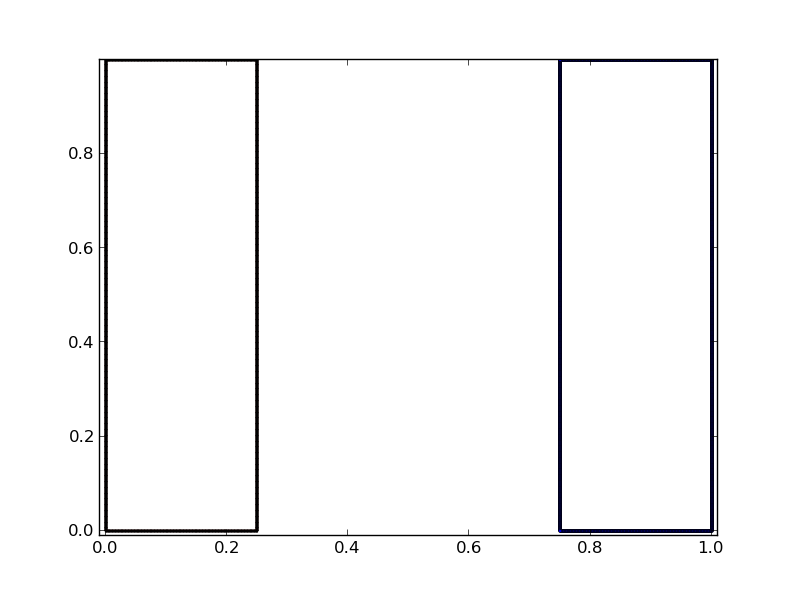
\includegraphics[width=0.45\textwidth]{horseshoe_v1}
    \hspace{2mm}
    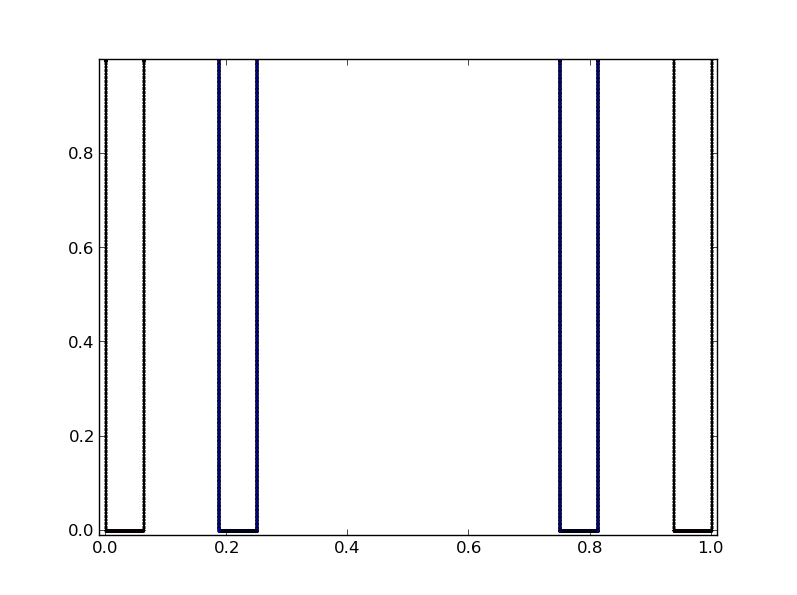
\includegraphics[width=0.45\textwidth]{horseshoe_v2}
    \vspace{2mm}
    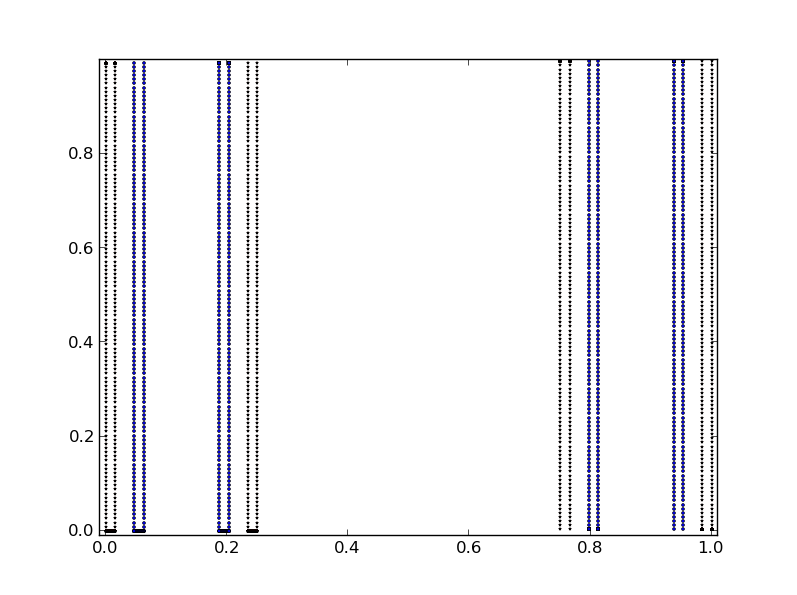
\includegraphics[width=0.45\textwidth]{horseshoe_v3}
  \caption{
    Iteration of the horseshoe map on vertical strips. Once, twice, and thrice.
    $\lambda = 0.25$, $\mu = 3.0$.
  }
  \label{fig:horseshoe-vertical}
\end{figure}

\begin{figure}[ht]
  \centering
    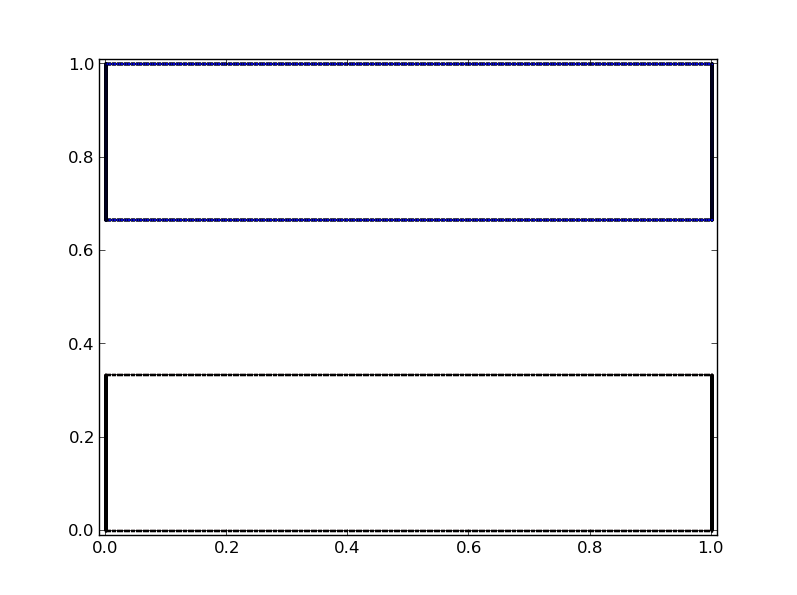
\includegraphics[width=0.45\textwidth]{horseshoe_h1}
    \hspace{2mm}
    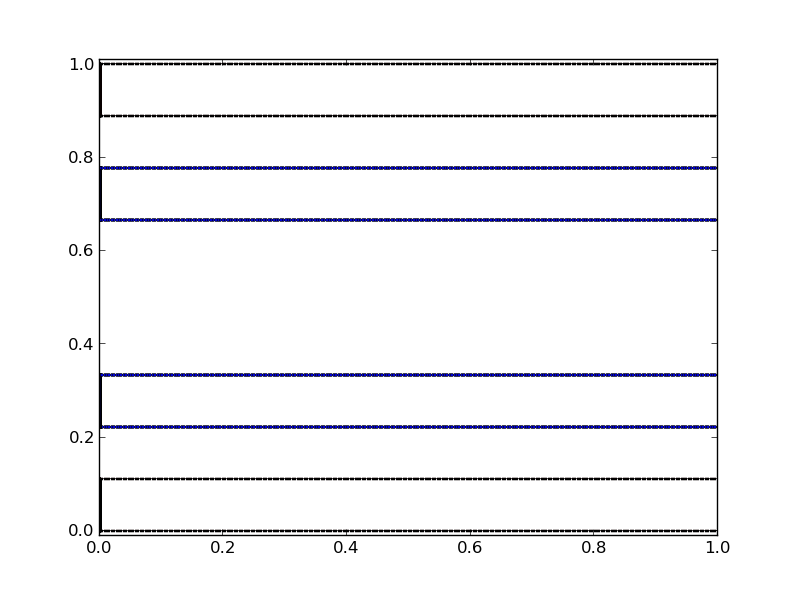
\includegraphics[width=0.45\textwidth]{horseshoe_h2}
    \hspace{2mm}
    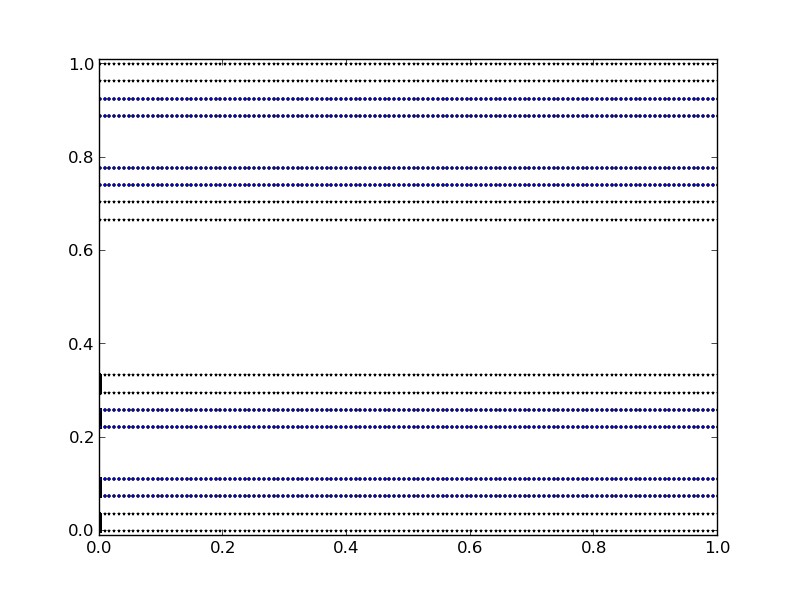
\includegraphics[width=0.45\textwidth]{horseshoe_h3}
  \caption{
    Iteration of the horseshoe map on horizontal strips. Once, twice, and thrice.
    $\lambda = 0.25$, $\mu = 3.0$.
  }
  \label{fig:horseshoe-horizontal}
\end{figure}

The \textit{invariant set} of the horseshoe map is a set $\Lambda$ such that $H(\Lambda) = \Lambda$.

The dynamics of the horseshoe map is (geometrically) complicated.
However, we can understand topological properties of the map by studying the dynamics of \textit{symbols}.
We will expound on this point in the next section.
Specifically, we will prove the following properties of $H$ and its invariant set:
\begin{enumerate}[(i)]
  \item $H$ has a countable infinity of periodic orbits of any period.
  \item $H$ has an uncountable infinity of non-periodic orbits.
  \item $H$ has a dense orbit (analogous to transitivity).
  \item $H$ has a \textit{sensitive dependence on initial condition} on its invariant set.
\end{enumerate}
%%%

\section{Two-Sided Shift}
As we mentioned in the previous section, ($D$, $H$) is conjugate to the \textit{two-sided shift} ($\Sigma$, $\sigma$), defined as follows.
\begin{definition}
  (Two-Sided Shift)
  Let $S$ be a set of finite number (at least 2) of symbols, and let $\Sigma$ be a set of bi-infinite sequences of the form
  \begin{equation*}
    s = \set{ \cdots s_{-n} \cdots s_{-1} * s_0 \cdots s_n \cdots },
  \end{equation*}
  where $s_i \in S$, and the asterisk is a placeholder to denote the 0th place (i.e. the symbol after $*$ is the 0th place).
  We often take a finite number of integers, $\set{1, \ldots, n}$ as our symbols.
  Define the metric on $\Sigma$ as follows:
  \begin{equation*}
    d(a,b) = \sum\limits_{i = -\infty}^{\infty} \frac{1}{2^{\abs{i}}} \frac{\abs{a_i - b_i}}{1 + \abs{a_i - b_i}}.
  \end{equation*}
  Let $\sigma: \Sigma \to \Sigma$ defined as:
  \begin{equation*}
    \sigma: \set{ \cdots s_{-n} \cdots s_{-2} s_{-1} * s_0 \cdots s_n \cdots } \mapsto \set{ \cdots s_{-n} \cdots s_{-2} * s_{-1} s_0 \cdots s_n \cdots }.
  \end{equation*}
  We call the dynamical system ($\Sigma$, $d$, $\sigma$) a \textit{two-sided shift}.
\end{definition}
Before we proceed further, we should first confirm that the definition makes sense.
\begin{proposition}
  $d$ is indeed a metric.
  \label{prop:symb-metric}
  \begin{proof}
    We only prove the triangle inequality.
    The other properties are trivial to show.
    Suppose $a,b,c \in \Sigma$.
    We have
    \begin{align*}
      d(a,b) + d(b,c)
      &= \sum\limits_{i = -\infty}^{\infty} \frac{1}{2^{\abs{i}}} \frac{\abs{a_i - b_i}}{1 + \abs{a_i - b_i}}
        +
        \sum\limits_{i = -\infty}^{\infty} \frac{1}{2^{\abs{i}}} \frac{\abs{b_i - c_i}}{1 + \abs{b_i - c_i}}   \\
      &= \sum\limits_{i = -\infty}^{\infty} \frac{1}{2^{\abs{i}}} \paren{ \frac{\abs{a_i - b_i}}{1 + \abs{a_i - b_i}} + \frac{\abs{b_i - c_i}}{1 + \abs{b_i - c_i}} }.
    \end{align*}
    To simplify notations, let $d_1 = \abs{a - b}$, $d_2 = \abs{b - c}$, $d_3 = \abs{a - c}$.
    We would like to show
    \begin{equation*}
      \frac{d_1}{1 + d_1} + \frac{d_2}{1 + d_2} \geq \frac{d_3}{1 + d_3},
    \end{equation*}
    which is equivalent to
    \begin{equation*}
      d_1(1+d_2)(1+d_3) + d_2(1+d_1)(1+d_3) \geq  d_3(1+d_1)(1+d_2).
    \end{equation*}
    Notice that
    \begin{align*}
      &d_1(1+d_2)(1+d_3) + d_2(1+d_1)(1+d_3) - d_3(1+d_1)(1+d_2)  \\
      &= (d_1 + d_2) - d_3 + 2d_1d_2 + d_1d_2d_3  \\
      &\geq 2d_1d_2 + d_1d_2d_3
    \end{align*}
    by $d_1 + d_2 \geq d_3$.
    This proves the triangle equality.
 \end{proof}
\end{proposition}
The metric defines the topology on $\Sigma$.

Now we need to check that $\sigma$ is continuous.
We first prove two useful properties of the metric.
\begin{proposition}
  \begin{enumerate}
    \item $d(a,b) < \frac{1}{2^{n+1}}$ implies $a_i = b_i$ for each $\abs{i} \leq n$.
    \item $a_i = b_i$ for each $\abs{i} \leq n$ implies $d(a,b) \leq \frac{1}{2^{n-1}}$.
  \end{enumerate}
  \begin{proof}
    (i) Proof by contradiction. Suppose there exists $\abs{j} \leq n$ such that $a_j \neq a_j$.
    Then, 
    \begin{align*}
      d(a,b) &\geq \frac{1}{2^j} \frac{\abs{a_j - b_j}}{1 + \abs{a_j - b_j}}  \\
      &\geq \frac{1}{2^j} \frac{1}{2}  \\
      &= \frac{1}{2^{j+1}}.
    \end{align*}
    This contradicts our hypothesis.  \\
    (ii) We have
    \begin{align*}
      d(a,b) &= \sum\limits_{i = -\infty}^{-(M+1)} \frac{1}{2^i} \frac{\abs{a_i - b_i}}{1 + \abs{a_i - b_i}}  +  \sum\limits_{i = M+1}^{\infty} \frac{1}{2^i} \frac{\abs{a_i - b_i}}{1 + \abs{a_i - b_i}}  \\
      &= 2 \sum\limits_{i = M+1}^{\infty} \frac{1}{2^i} \frac{\abs{a_i - b_i}}{1 + \abs{a_i - b_i}}  \\
      &\leq 2 \sum\limits_{i = M+1}^{\infty} \frac{1}{2^i} \cdot 1  \\
      &= \sum\limits_{i = M+1}^{\infty} \frac{1}{2^{i-1}}   \\
      &= \frac{1}{2^{i-1}}.
    \end{align*}
  \end{proof}
\end{proposition}
Other properties of $\sigma$ are also easy to see.
\begin{proposition}
  ($\sigma$ is a homeomorphism)
  \begin{enumerate}[(i)]
    \item $\sigma$ is continuous.
    \item  $\sigma$ is surjective.
    \item  $\sigma$ is injective.
  \end{enumerate}
  \begin{proof}
    (i)
    Fix $\delta > 0$ and $a \in \Sigma$, and suppose that $\delta \geq \frac{1}{2^{n-3}}$ for some $n$.
    We want to find an $\epsilon$ such that $b \in \oball{\epsilon}{a}$ implies $\sigma(b) \in \oball{\delta}{\sigma(a)}$.
    Let $\epsilon = \frac{1}{2^{n+1}}$.
    Then, by the lemma, $a_i = b_i$ for $\abs{i} \leq n$.
    It follows that $\sigma(a_i) = \sigma(b_i)$ for $\abs{i} \leq n-1$.
    By the lemma, we have $d(\sigma(a), \sigma(b)) \leq \frac{1}{2^{n-2}} \leq \delta$.  \\
    (ii) For each $a \in \Sigma$, $\sigma^{-1}(a)$ is nonempty.  \\
    (iii) This is trivial.
  \end{proof}
  \label{prop:symb-sigma-cont}
\end{proposition}
\begin{proposition}
\end{proposition}
\begin{proposition}
\end{proposition}
Note the following properies of $S$, the set of finite symbols.
\begin{proposition}
  $S$ equipped with the absolute value metric is compact, totally disconnected, and perfect.
\begin{proof}
  (Compactness)
  
  (Totally disconnectedness)

  (Perfectness)

\end{proof}
\end{proposition}
These properties of the underlying space are inherited to the space of bi-infinite sequences of symbols, $\Sigma$, since $\Sigma \equiv \prod\limits_{i = -\infty}^{\infty} S$, where $\prod$ denotes cartesian product.
The precise statement is the following proposition.
\begin{proposition}
  $\Sigma$ equipped with the metric $d$ is compact, totally disconnected, and perfect.
\begin{proof}
  (Compactness)
  
  (Totally disconnectedness)

  (Perfectness)

\end{proof}
\end{proposition}
\begin{proposition}
  Compactness, connectedness, and perfectness are topological properties (i.e. preserved under continuous mappings)
\end{proposition}

In this section, we use $S = \set{0,1}$, so that an element of $\Sigma$ is a bi-infinite sequence of 0 and 1.
To gain some insights of the dynamics of the two-sided shift, we shall spend some time on discussing what $d$ and $\sigma$ are.
If $S = \set{0,1}$, then the metric on $d$ can be written as
\begin{equation*}
  d(a,b) = \sum\limits_{i = -\infty}^{\infty} \frac{1}{2^{\abs{i}}} \delta_{i},
\end{equation*}
where
\begin{equation*}
  \delta = 
  \begin{cases}
    &0 \quad \mbox{ if } a_i = b_i  \\
    &1 \quad \mbox{ otherwise.}
  \end{cases}
\end{equation*}
Thus, two bi-infinite sequences are ``close'' to each other if they agree on a long central block.
Also, we can think of a bi-infinite sequence in $\Sigma$ as a binary expansion of some real number, and think of $*$ as a symbol that separates the fractional part (before $*$) from integer part (after $*$).
In this scheme, $\sigma$ corresponds to multiplication of a binary number by $2$.

As a consequence, ($D$, $H$) possesses any topological property of ($\Sigma$, $\sigma$), and vice versa.

%\begin{theorem}
%  (Conley-Moser Condition)
%  Suppose $F$ satisfies the following two conditions.
%  \begin{enumerate}
%    \item $F(H_i) = V_i$ for each $1 \leq i \leq n$.
%          Moreover, $F$ maps the horizontal boundaries of $H_i$ to the horizontal boundaries of $V_i$, and the vertical boundaries of $H_i$ to the vertical boundaries of $V_i$.
%    \item If $H$ is a $\mu_h$-horizontal strip contained in $\bigcup_{i} H_i$, then $F^{-1}(H) \cap H_i$ is a $\mu_h$-horizontal strip for every $i$.
%          Moreover, $d(F^{-1}(H) \cap H_i) \leq \nu_h d(H)$ for some $0 < \nu_h < 1$.
%    \item The same condition for $\mu_v$-vertical strips.
%  \end{enumerate}
%  \label{thm:conley-moser}
%\end{theorem}


